\documentclass[10pt,conference]{IEEEtran}
\IEEEoverridecommandlockouts
\usepackage{cite}
\usepackage{amsmath,amssymb,amsfonts}
\usepackage{algorithmic}
\usepackage{graphicx}
\usepackage{textcomp}
\usepackage{xcolor}
\usepackage{booktabs}
\usepackage{url}

% ============================================================
% DRAFT NOTE (remove before submission):
% Numbers rendered with \FIX{...} are PLACEHOLDERS to be
% replaced with measured values from the actual experimental
% runs. They are NOT results; do not submit with red text.
% ============================================================
\newcommand{\FIX}[1]{\textcolor{red}{#1}}

\def\BibTeX{{\rm B\kern-.05em{\sc i\kern-.025em b}\kern-.08em
    T\kern-.1667em\lower.7ex\hbox{E}\kern-.125emX}}

\begin{document}

\title{MARQ: Structured Multi-Agent Reasoning for\\ Ambiguity Defect Detection in Software Requirements}

\author{\IEEEauthorblockN{Anonymous Author(s)}
\IEEEauthorblockA{\textit{Affiliation omitted for double-anonymous review}}
}

\maketitle

\begin{abstract}
Detecting ambiguity defects in natural-language requirements is a core quality-assurance task. Existing language-model approaches are typically evaluated in a simplified setting, in which the specific weak word to inspect is supplied to the model. Real reviewers receive no such hint: they must first locate what might be problematic and only then judge it. We reformulate the task to this harder, requirement-level setting, in which the model sees only the requirement text, and we argue that it exposes properties that monolithic prompting cannot satisfy in principle: the task combines a recall-oriented location subtask with a precision-oriented judgment subtask, and its intermediate verdicts benefit from verification whose errors are decorrelated from the generator. Motivated by these properties, we introduce MARQ, a training-free multi-agent system that separates location, judgment, adversarial critique, and aggregation across specialized agents over small open language models. In this short study we test a single hypothesis: that structured multi-agent reasoning outperforms monolithic single-trajectory prompting under the hint-free setting. We describe the architecture, its motivation, and a controlled comparison against zero-shot, few-shot, and chain-of-thought baselines across several small open models, and we outline the plan to develop these emerging results into a full study.
\end{abstract}

\begin{IEEEkeywords}
requirements engineering, ambiguity detection, large language models, multi-agent systems, natural-language processing
\end{IEEEkeywords}

\section{Introduction}
Natural-language requirements remain the dominant medium for specifying software, and ambiguity in them is a well-documented source of downstream defects. A requirement such as ``the system shall process the incoming request quickly and return an appropriate response'' contains at least two under-specified expressions, ``quickly'' and ``appropriate'', either of which a reviewer may flag as a quality defect. Automating this review is attractive, and recent work applies large language models (LLMs) to requirements quality classification with encouraging accuracy.

However, a gap separates how these methods are evaluated from how requirements review actually happens. Benchmarks such as QuRE~\cite{qure} provide labeled tuples of the form \emph{(requirement, weak\_word)}~$\rightarrow$~\emph{ok/defect}: the model is \emph{told} which word to assess. A human reviewer is not. This simplification quietly removes the hardest half of the task, namely deciding \emph{where} in a requirement a problem might lie before deciding \emph{whether} it is one.

We reformulate ambiguity defect detection to the requirement level and remove the hint: at inference time a method receives only the requirement text. Our position, developed in Sections~\ref{sec:problem} and~\ref{sec:example}, is that this reformulated task has properties a single reasoning trajectory cannot satisfy. It couples a recall-oriented \emph{location} subtask with a precision-oriented \emph{judgment} subtask, two goals with opposite optimal operating points; and its intermediate verdicts benefit from \emph{decorrelated} verification, which sampling many trajectories from one model (as in self-consistency) does not provide. These are properties of the problem, not of any model, and they motivate decomposition into specialized, communicating agents rather than a more elaborate prompt.

Guided by these properties, we introduce \textbf{MARQ} (Multi-Agent Reasoning for requirements Quality), a training-free system in which a retriever, a scanner, per-concern investigators, an adversarial critic, and a synthesizer each own one reasoning activity, over small open LLMs runnable on a single consumer GPU. As an emerging-results study, this paper tests one hypothesis:

\begin{quote}
\textbf{RQ1.} Under the hint-free, requirement-level setting, does structured multi-agent reasoning (MARQ) outperform monolithic single-trajectory prompting (zero-shot, few-shot, chain-of-thought)?
\end{quote}

RQ1 is the minimal claim that justifies the architecture: if simpler prompting already sufficed, the added complexity would be unwarranted. We contribute (i) the hint-free task reformulation; (ii) the MARQ architecture together with a first-principles motivation for its decomposition; and (iii) a controlled RQ1 comparison across several small open models. Broader questions of generality, cost, and benchmark auditing are deferred to a full study, outlined in Section~\ref{sec:future}.

\section{Problem}
\label{sec:problem}
Automated requirements review increasingly relies on LLMs, but the way these methods are evaluated diverges from how review actually happens, and closing that gap changes the nature of the task.

\paragraph*{Ambiguity defects and QuRE}
Requirements ``smells''---linguistic indicators of potential quality problems such as vague terms, comparatives without a reference, and loopholes---have long served as lightweight quality signals~\cite{smells}. QuRE~\cite{qure} operationalizes a subset of these as an annotated benchmark of industrial requirements, in which each candidate weak word carries an \emph{ok}/\emph{defect} label established through human review. Prior LLM-based work, including prompt-engineering studies over the same data, has largely adopted this word-level framing~\cite{ape_anon}.

\paragraph*{From word-level hints to requirement-level review}
Let a requirement $r$ carry annotated weak-word instances $w_1,\dots,w_m$ with per-instance labels $y_i\in\{\text{ok},\text{defect}\}$. We define the requirement-level label
\[
Y(r) = \text{defect} \iff \exists i:\, y_i = \text{defect},
\]
and \emph{ok} otherwise. At inference, a method observes only the text of $r$; weak-word annotations and per-word labels exist only inside a labeled example pool used for in-context learning, never for the test item. This mirrors real review, where the reviewer must surface candidate problems unaided.

\paragraph*{Coupled sub-objectives}
Removing the hint splits the task into locating candidate ambiguous expressions and judging each in context. Location is a recall problem: a missed span guarantees a wrong requirement-level label. Judgment is a precision problem: flagging every hedge word destroys accuracy. A single prompt exposes one instruction set and one effective operating point, and therefore cannot be simultaneously recall-oriented in location and precision-oriented in judgment.

\paragraph*{Limits of monolithic prompting}
A natural response is that a stronger prompt, or chain-of-thought (CoT)~\cite{cot} with self-consistency~\cite{selfcons}, should suffice. CoT keeps a model on one reasoning trajectory; self-consistency samples many trajectories from the \emph{same} distribution and votes, reducing variance but not systematic bias, so correlated errors survive the vote. Catching a confidently wrong verdict instead requires an assessment whose errors are \emph{decorrelated} from the generator's---an independently prompted critic that did not produce the original verdict and is not anchored to it. The hypothesis under test is therefore not that ``more reasoning'' helps, but that \emph{structured, independently verified} reasoning is better matched to this task than a single prompt, however engineered.

\section{Motivating Example}
\label{sec:example}
Consider again the requirement ``the system shall process the incoming request quickly and return an appropriate response.'' Under QuRE the model would be handed one of the words ``quickly'' or ``appropriate'' and asked only to rate it; under our setting it receives the sentence alone.

A human reviewer does not decide ``ambiguous / not ambiguous'' in one step. They \emph{scan} the sentence for under-specified expressions, surfacing ``quickly'' and ``appropriate'' (and perhaps considering, then discarding, ``the user''). They \emph{assess} each candidate separately in context: ``quickly'' has no bound or reference workload and is likely defective, whereas ``appropriate response'' may be acceptable if an earlier requirement defines the response set, so its verdict is conditional. They \emph{challenge} inconclusive readings---is ``quickly'' constrained by a non-functional requirement elsewhere; is ``appropriate'' a defined term---actively trying to falsify a first impression. Finally they \emph{integrate} the surviving concerns: any unresolved ambiguity makes the requirement a defect.

Each step is exactly where one of the difficulties from Section~\ref{sec:problem} bites: scanning is the recall-oriented location subtask, per-concern assessment is precision-oriented judgment under isolation, challenging is decorrelated verification, and integration is a simple aggregation rule. This paper therefore addresses the following problem: \emph{how can we detect ambiguity defects from requirement text alone, in a way that separates locating from judging and verifies intermediate verdicts before committing to a label?}

\section{Vision: Structured Multi-Agent Reasoning}
\label{sec:vision}
Our approach realizes the reviewer's process as a set of specialized agents. Crucially, the motivation is not that imitating humans is inherently correct, but that the decomposition secures the three properties above---separating recall from precision, isolating per-concern judgments, and inserting decorrelated verification---which no monolithic prompt provides. All agents are instances of the same small open LLM, differentiated only by role prompts; no weights are updated.

\subsection{From Reviewer Reasoning to Specialized Agents}
We map the four reviewing activities onto agents and add a deterministic grounding step. Scanning becomes a recall-oriented \emph{Scanner}; per-concern assessment becomes parallel \emph{Investigators}, one per concern, each reasoning in isolation; challenging becomes an adversarial \emph{Critic} whose errors are decorrelated from the generators'; integration becomes a transparent \emph{Synthesizer}. Because the hint that would tell a method what ``weak'' looks like is withheld, a \emph{Retriever} supplies that signal from data by fetching labeled examples similar to the requirement under review.

\subsection{The MARQ Pipeline}
The five roles operate over a shared example pool (Fig.~\ref{fig:arch}):

\begin{itemize}
\item \textbf{Retriever} (deterministic): dense top-$k$ retrieval over the labeled pool using sentence embeddings~\cite{sbert}, returning $k$ requirement-level examples with their annotations.
\item \textbf{Scanner} (recall): reads the requirement and retrieved examples and emits candidate ambiguity concerns as spans with reasons, instructed to favor recall; precision is deferred.
\item \textbf{Investigator} (one per concern, parallel): judges a single concern as grounded or vague in context, returning a verdict, a confidence, and a rationale, isolated from sibling concerns.
\item \textbf{Critic} (verification): adversarially reviews the collected verdicts, challenging low-confidence judgments and those contradicting retrieved examples, and may trigger one bounded re-investigation round.
\item \textbf{Synthesizer}: applies the aggregation rule (any surviving defect $\Rightarrow$ defect) and emits the final label plus a natural-language rationale.
\end{itemize}

A prediction costs typically three to six LLM calls; this overhead is the price of the properties above and is measured explicitly in the full study. Every method---baselines and MARQ alike---emits a reasoning string per prediction, logged for analysis. This design adapts insights from multi-agent debate~\cite{debate}, self-refinement~\cite{selfrefine}, and LLM-as-judge evaluation~\cite{judge} to a requirements task, with an explicit location/judgment split grounded in retrieval.

\begin{figure}[t]
\centerline{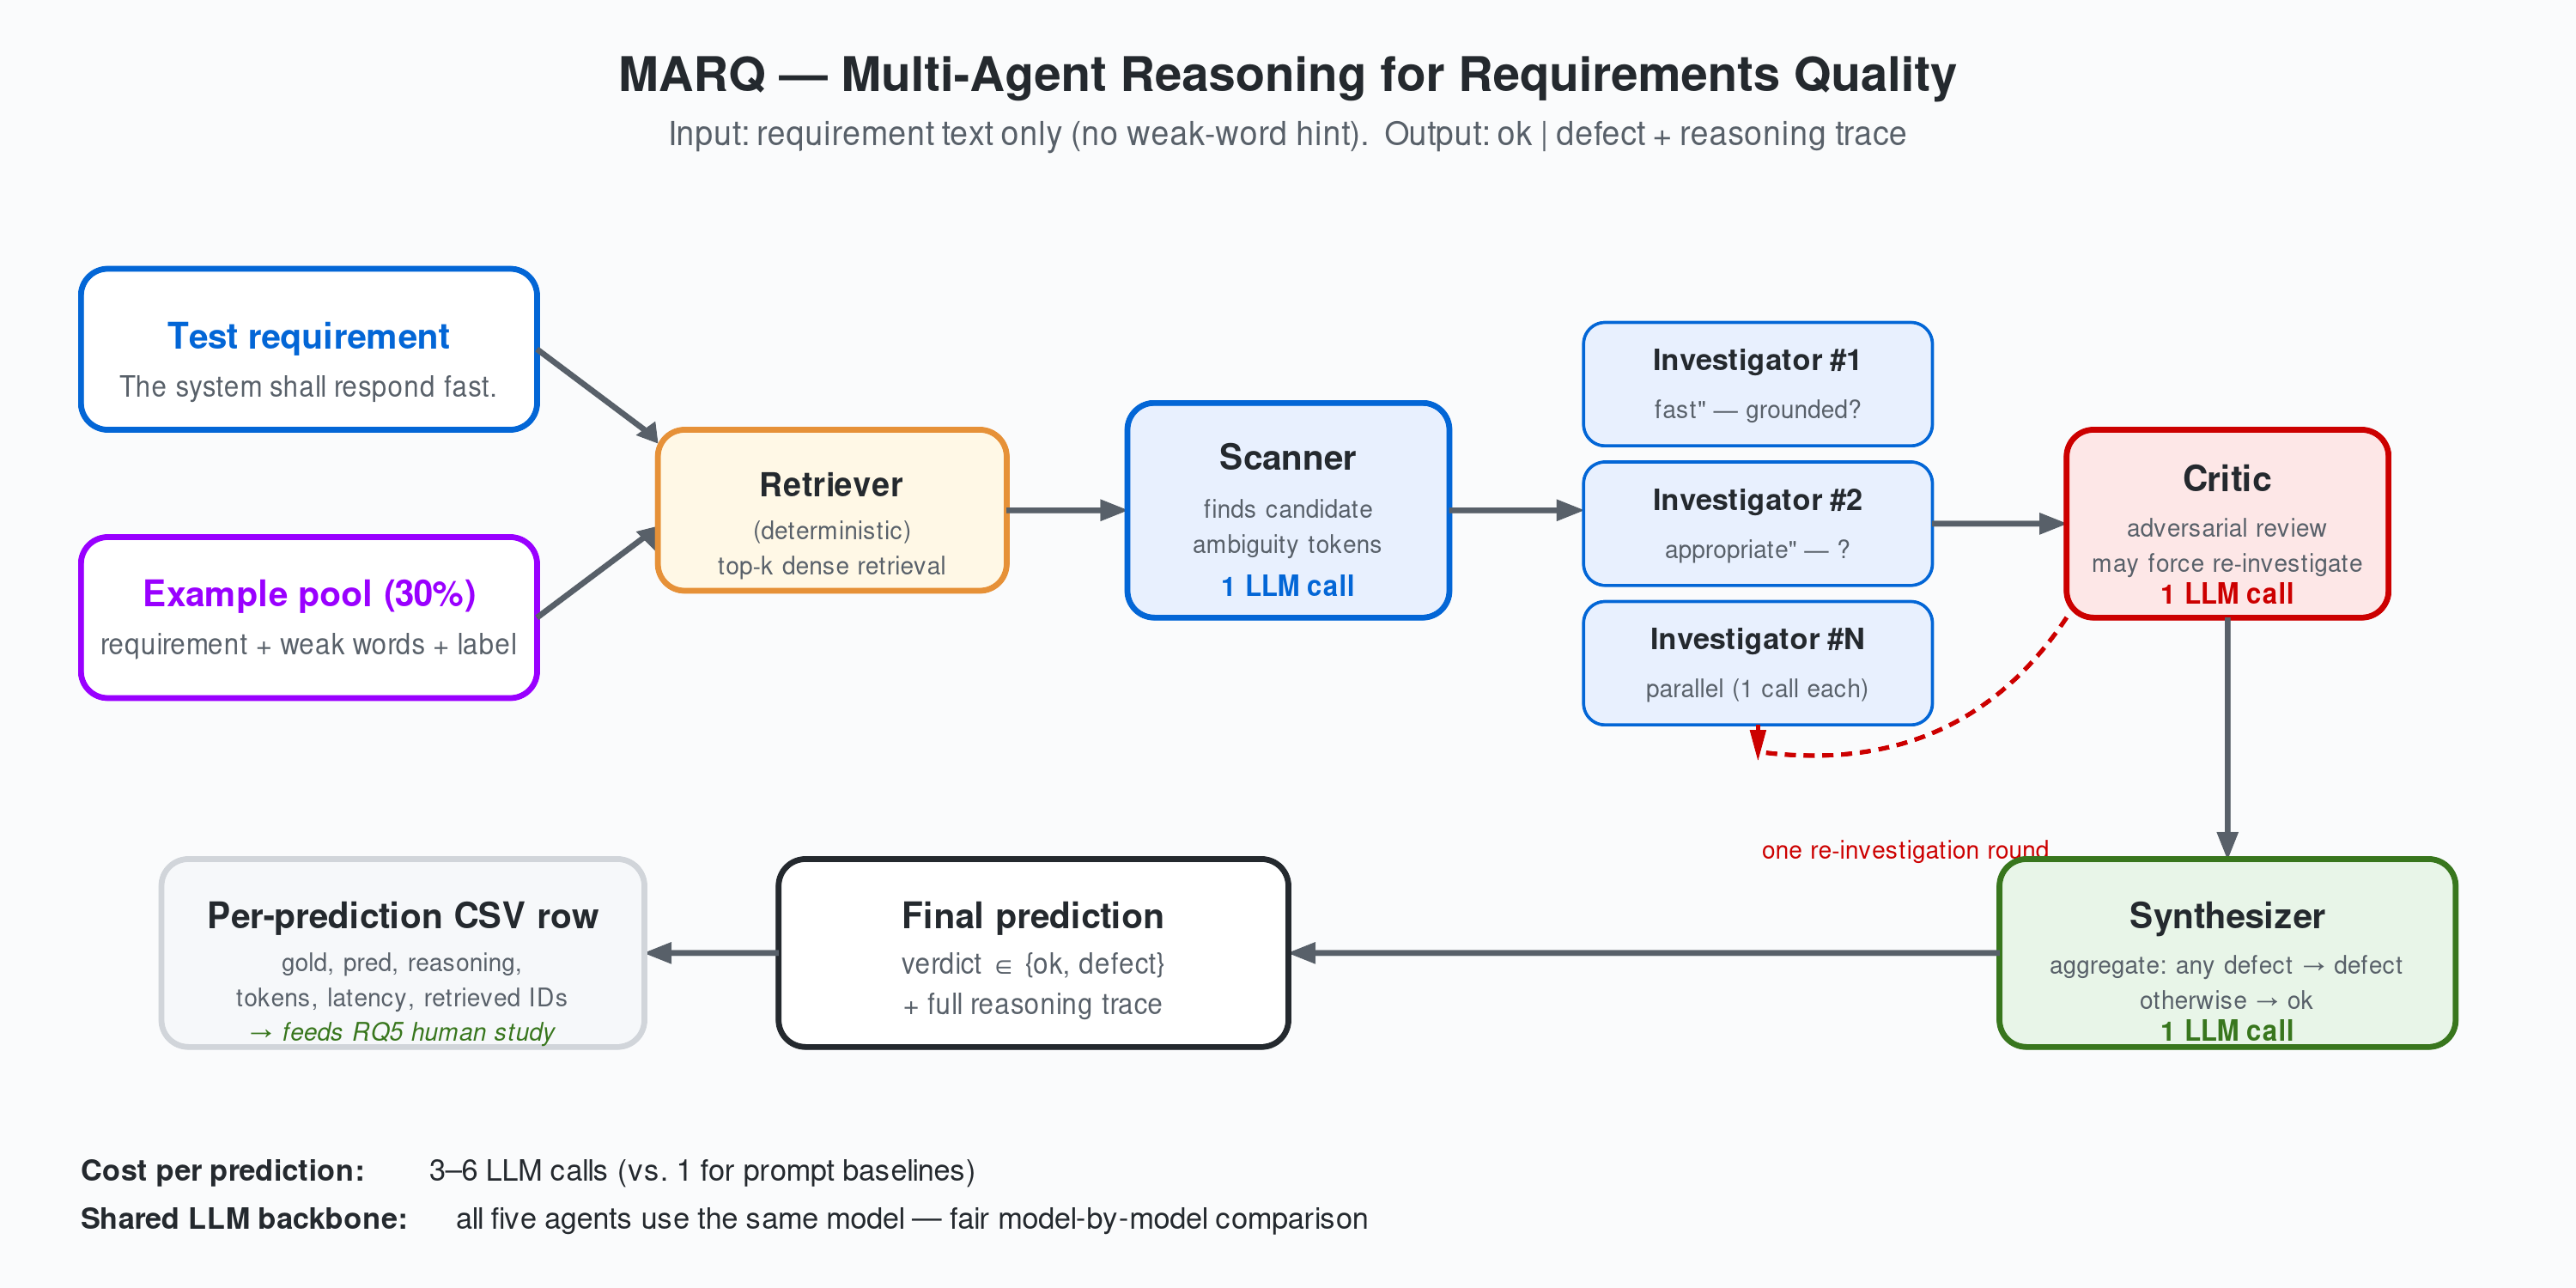
\includegraphics[width=\columnwidth]{architecture.png}}
\caption{MARQ pipeline. A deterministic retriever grounds a recall-oriented scanner; per-concern investigators judge in isolation; an adversarial critic triggers bounded revision; a synthesizer aggregates surviving verdicts into a final label and rationale.}
\label{fig:arch}
\end{figure}

\section{Study Design}
\label{sec:design}
\subsection{Data and protocol}
We use QuRE~\cite{qure} under the reformulation of Section~\ref{sec:problem}. Because we introduce no separate validation split, we adopt repeated stratified holdout: \texttt{StratifiedShuffleSplit} with five folds, each a 30\%/70\% pool/test partition stratified on the requirement-level label. The 30\% pool is the only labeled resource visible to any method (as the in-context retrieval source); the 70\% test set is scored on requirement text alone. All hyperparameters ($k{=}5$ retrieval, prompt wording, agent loop bounds) are fixed once, before any runs, and held constant across folds; we do not tune on folds. Results are reported as mean~$\pm$~standard deviation across the five folds.

\subsection{Baselines}
All baselines are single-agent and receive the same retrieved pool where applicable, isolating the effect of \emph{structure}: \emph{Zero-shot} (one call, brief rationale requested); \emph{Few-shot} ($k{=}5$ retrieved examples with their annotations, one call); and \emph{CoT few-shot} (same examples, each carrying a one-sentence reasoning chain, with an explicit step-by-step instruction, one call).

\subsection{Models}
To separate the effect of structure from model capacity, we run every method on several small open instruction-tuned models spanning three size classes and four families, all runnable on a single consumer GPU: Qwen2.5-1.5B and Qwen2.5-7B~\cite{qwen}, Llama-3.2-3B~\cite{llama}, Gemma-2-2B~\cite{gemma}, and Phi-3.5-mini~\cite{phi}.

\subsection{Metrics}
The primary metric is macro-$F_1$ over the \emph{defect}/\emph{ok} labels, with precision and recall reported for the \emph{defect} class given the class imbalance. We accompany point estimates with bootstrap confidence intervals and test MARQ against the strongest baseline per model using McNemar's test on paired predictions. Following community guidance on sustainable evaluation, we also record LLM calls and tokens per prediction as cost context.

\section{Preliminary Results and Discussion}
\label{sec:results}
% ---------------------------------------------------------------
% PLACEHOLDER RESULTS. Replace every \FIX{...} value below with
% measured numbers from run_evaluation.py before submission.
% Do NOT submit with red placeholder text present.
% ---------------------------------------------------------------
Table~\ref{tab:main} reports macro-$F_1$ per model for each method (mean over five folds). \emph{The values shown are placeholders pending the final run and must be replaced with measured results.}

\begin{table}[t]
\caption{Macro-$F_1$ (mean over five folds) under the hint-free requirement-level setting. Placeholder values; to be replaced with measured results.}
\label{tab:main}
\begin{center}
\begin{tabular}{lcccc}
\toprule
\textbf{Model} & \textbf{Zero} & \textbf{Few} & \textbf{CoT} & \textbf{MARQ} \\
\midrule
Qwen2.5-1.5B & \FIX{.xx} & \FIX{.xx} & \FIX{.xx} & \FIX{.xx} \\
Gemma-2-2B   & \FIX{.xx} & \FIX{.xx} & \FIX{.xx} & \FIX{.xx} \\
Llama-3.2-3B & \FIX{.xx} & \FIX{.xx} & \FIX{.xx} & \FIX{.xx} \\
Phi-3.5-mini & \FIX{.xx} & \FIX{.xx} & \FIX{.xx} & \FIX{.xx} \\
Qwen2.5-7B   & \FIX{.xx} & \FIX{.xx} & \FIX{.xx} & \FIX{.xx} \\
\midrule
Mean         & \FIX{.xx} & \FIX{.xx} & \FIX{.xx} & \FIX{.xx} \\
\bottomrule
\end{tabular}
\end{center}
\end{table}

We report three observations against RQ1: whether MARQ attains the highest mean macro-$F_1$ and on how many models its improvement over the strongest baseline is significant under McNemar's test; whether the gain concentrates on \emph{recall} for the \emph{defect} class, consistent with the scanner surfacing problems that single-call methods miss; and whether the critic's re-investigation flips a measurable fraction of low-confidence verdicts, consistent with decorrelated verification. The claim under test is deliberately narrow: that \emph{structure}, not capacity or prompt wording, drives any difference.

\paragraph*{Threats to validity}
The requirement-level label is a disjunction over human-annotated weak words; residual annotation noise in QuRE bounds achievable accuracy but affects all methods equally---an issue we turn into a research question in the full study. All methods share the same retrieved pool and fixed hyperparameters, so observed differences are attributable to structure rather than tuning; agent prompts were nonetheless authored by us and could favor MARQ, a risk we mitigate by fixing and releasing them before runs. Results are limited to one benchmark and five small open models, and five folds is modest; we report variance and paired significance tests rather than point estimates alone, and defer broader generality to the full study.

\section{Future Plans}
\label{sec:future}
This paper reports the emerging result that structured multi-agent reasoning can outperform monolithic prompting on hint-free requirement quality review (RQ1). To turn it into a full-length paper we plan five extensions. First, we will \emph{harden the comparison} by adding CoT with self-consistency and a two-stage ``locate-then-judge'' single-agent prompt as baselines, so that the benefit of multi-agent structure cannot be attributed to reasoning depth or trajectory voting alone. Second, we will study \emph{generality}: scaling across model sizes and additional families, and, resources permitting, a second requirements dataset. Third, we will run \emph{ablations} that remove each agent (critic, scanner, retrieval) to quantify its marginal contribution. Fourth, we will characterize the \emph{cost--quality trade-off}, reporting tokens, latency, and estimated energy per prediction to locate MARQ on a Pareto frontier and assess industrial applicability. Fifth, and most ambitiously, we will use the per-prediction reasoning traces to \emph{audit the benchmark}: where model verdicts systematically disagree with QuRE's gold labels, we will run a blind human study to adjudicate which is correct, quantifying label noise and proposing a cleaned subset. Together these turn a single confirmatory result into an evaluation of when structured reasoning is worth its overhead and what it reveals about the data.

\section*{Sustainability Note}
MARQ trades additional inference calls for accuracy, so its environmental cost is non-trivial and should be reported rather than hidden. All models are small enough to run on a single consumer GPU, avoiding training and large-model serving costs; we log LLM calls and token counts per prediction and will report estimated energy per prediction in the full study, enabling practitioners to weigh accuracy against footprint.

\section*{Data Availability}
In line with ICSE open-science expectations, the code, prompts, fold splits, and per-prediction reasoning logs will be released in an anonymized repository upon acceptance.

\begin{thebibliography}{00}
\bibitem{qure} H. Femmer et al., ``QuRE: A benchmark for requirements quality defect detection,'' in \emph{Proc. IEEE Int. Requirements Eng. Conf. Workshops (REW)}, 2025.
\bibitem{smells} H. Femmer, D. Mendez Fern\'andez, S. Wagner, and S. Eder, ``Rapid quality assurance with requirements smells,'' \emph{J. Syst. Softw.}, vol. 123, pp. 190--213, 2017.
\bibitem{ape_anon} Anonymized, ``Automatic prompt engineering for requirements classification,'' 2025, citation omitted for double-anonymous review.
\bibitem{cot} J. Wei et al., ``Chain-of-thought prompting elicits reasoning in large language models,'' in \emph{Adv. Neural Inf. Process. Syst. (NeurIPS)}, 2022.
\bibitem{selfcons} X. Wang et al., ``Self-consistency improves chain of thought reasoning in language models,'' in \emph{Int. Conf. Learn. Representations (ICLR)}, 2023.
\bibitem{debate} Y. Du, S. Li, A. Torralba, J. B. Tenenbaum, and I. Mordatch, ``Improving factuality and reasoning in language models through multiagent debate,'' in \emph{Proc. Int. Conf. Mach. Learn. (ICML)}, 2024.
\bibitem{selfrefine} A. Madaan et al., ``Self-refine: Iterative refinement with self-feedback,'' in \emph{Adv. Neural Inf. Process. Syst. (NeurIPS)}, 2023.
\bibitem{judge} L. Zheng et al., ``Judging LLM-as-a-judge with MT-bench and chatbot arena,'' in \emph{Adv. Neural Inf. Process. Syst. (NeurIPS)}, 2023.
\bibitem{sbert} N. Reimers and I. Gurevych, ``Sentence-BERT: Sentence embeddings using Siamese BERT-networks,'' in \emph{Proc. Conf. Empirical Methods Nat. Lang. Process. (EMNLP)}, 2019.
\bibitem{qwen} A. Yang et al., ``Qwen2.5 technical report,'' arXiv:2412.15115, 2024.
\bibitem{llama} A. Dubey et al., ``The Llama 3 herd of models,'' arXiv:2407.21783, 2024.
\bibitem{gemma} Gemma Team, ``Gemma 2: Improving open language models at a practical size,'' arXiv:2408.00118, 2024.
\bibitem{phi} M. Abdin et al., ``Phi-3 technical report: A highly capable language model locally on your phone,'' arXiv:2404.14219, 2024.
\end{thebibliography}

\end{document}
